% experiments_compact.tex — §6 Experiments (compact 9-page version)

\subsection{\method{} Evaluation on GSM8K}
\label{sec:town-eval}

We now verify the analytical predictions of \S\ref{sec:method} empirically.
\method{} (Algorithm~\ref{alg:town}) is evaluated with $B_1{=}256$, $B_2{=}512$ on the full GSM8K test set ($n{=}1{,}319$, Qwen3-8B).
Stage~1 resolves 88.8\% of samples (1,171/1,319) with 94.4\% accuracy at ${\sim}$133 avg tokens; the remaining 148 samples are routed to Stage~2, where thinking achieves 62.8\% on this hard subset.
Table~\ref{tab:town-comparison} compares \method{} against single-mode baselines.

\begin{table}[t]
\centering
\caption{\textbf{\method{} vs.\ single-mode baselines} on GSM8K ($n{=}1{,}319$, Qwen3-8B).
Thinking mode reaches parity with non-thinking only at budget 2048 (both 93.4\%), but requires 736 avg tokens vs.\ 152---a 4.8$\times$ cost.
\method{} achieves 90.9\% at 199 avg tokens, Pareto-dominating both its component baselines (\texttt{nothink@256} and \texttt{think@512}).
Note that \texttt{nothink@512} achieves higher accuracy (93.4\%) at fewer tokens (152); \method{} is designed for the regime where only $B_1$ tokens are affordable for most queries, with $B_2$ reserved for the hard subset.}
\label{tab:town-comparison}
\small
\begin{tabular}{lrrrr}
\toprule
\textbf{Strategy} & \textbf{Accuracy} & \textbf{Avg Tokens} & \textbf{Efficiency} & \textbf{$\Delta$ vs think@512} \\
\midrule
\texttt{think@256} & 18.0\% & 255 & 0.07\%/tok & $-$47.2pp \\
\texttt{think@512} & 65.2\% \ci{62.6}{67.8} & 477 & 0.14\%/tok & --- \\
\texttt{think@1024} & 86.8\% & 624 & 0.14\%/tok & +21.6pp \\
\texttt{think@2048} & 93.4\% & 736 & 0.13\%/tok & +28.2pp \\
\midrule
\texttt{nothink@256} & 87.5\% & 146 & 0.60\%/tok & +22.3pp \\
\texttt{nothink@512} & 93.4\% \ci{92.0}{94.7} & 152 & \textbf{0.61\%/tok} & +28.2pp \\
\midrule
\textbf{\method{} (ours)} & \textbf{90.9\%} \ci{89.3}{92.4} & \textbf{199} & 0.46\%/tok & \textbf{+25.7pp} \\
\bottomrule
\end{tabular}
\vspace{-2mm}
\end{table}

\method{} is \textbf{+25.7\,pp} more accurate than \texttt{think@512} at \textbf{2.3$\times$ fewer tokens}, and gains \textbf{+3.4\,pp} over \texttt{nothink@256} by recovering 64 genuinely hard cases (19 routing regrets; net +45 gains).

\paragraph{Error analysis.}
Of the 148 routed samples, 93 are correctly answered by thinking.
Among these, \textbf{64 are genuine recoveries} (nothink wrong, thinking correct) and 29 were correct in both modes.
However, \textbf{19 samples} exhibit routing regret: nothink produced a correct answer despite hitting the budget, but the thinking fallback answered incorrectly (1.4\% of all samples).
The remaining 36 routed samples were incorrect in both modes.
\method{}'s early-stop routing is optimal within the class of budget-utilization-based routers: it matches the token-length router exactly---providing a principled \emph{explanation} for why budget exhaustion is the right routing signal---and outperforms random (+5.9\,pp) and inverse-length (+7.4\,pp) baselines (Appendix~\ref{app:routing-baselines}).

\subsection{Crossover Analysis}
\label{sec:crossover}

\begin{figure}[t]
\centering
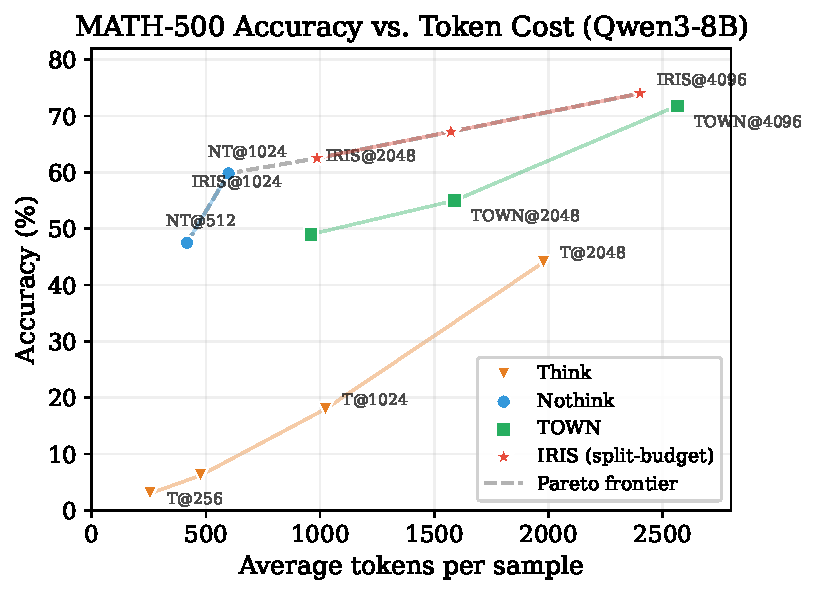
\includegraphics[width=\linewidth]{fig_pareto_frontier.pdf}
\vspace{-4mm}
\caption{\textbf{Cost-accuracy Pareto frontier} on GSM8K (left) and MATH-500 (right).
Non-thinking mode (blue) dominates thinking mode (red) at all tested budgets ($\leq$2048).
\method{} (green star) achieves the best accuracy-per-token tradeoff on GSM8K.
The crossover at ${\sim}$2048 tokens on GSM8K requires a 4$\times$ budget multiplier; on MATH-500, thinking has not yet reached parity at $b{=}2048$.}
\label{fig:pareto}
\vspace{-2mm}
\end{figure}

Figure~\ref{fig:pareto} reveals the cost-accuracy Pareto frontier.
On GSM8K, the crossover occurs at budget 2048 (both 93.4\%), requiring a \textbf{4$\times$ budget multiplier} over non-thinking's saturation point (512 tokens).
On MATH-500, the tax is even more severe: at budget 256, \emph{every single} thinking response is truncated (0\% natural stop, 0\% with final answer), yielding just 4.2\% accuracy.
At budget 1024, non-thinking achieves 59.8\% vs.\ thinking's 18.0\% (\textbf{41.8\,pp} gap, $p < 0.001$); even at 2048, thinking (44.0\%) trails non-thinking (64.4\%) by 20.4\,pp---the crossover has not been reached.
This non-convergence is arguably the most practically relevant finding: for challenging reasoning tasks, the thinking tax may persist across the \emph{entire practical budget range}, making adaptive routing not merely efficient but necessary.
Table~\ref{tab:math500-tax} provides the full MATH-500 budget sweep; per-difficulty-level breakdowns and complete data tables are in Appendices~\ref{app:math500-level} and \ref{app:full-tables}.

\begin{table}[t]
\centering
\caption{\textbf{Thinking tax on MATH-500} ($n{=}500$, Qwen3-8B).
Non-thinking mode outperforms thinking at \emph{every} tested budget ($\leq$2048), with the gap exceeding 20\,pp even at the highest budget.
The crossover has not been reached at $b{=}2048$, confirming harder benchmarks push it further right.}
\label{tab:math500-tax}
\small
\begin{tabular}{rrrr}
\toprule
\textbf{Budget} & \textbf{Nothink Acc} & \textbf{Think Acc} & \textbf{Gap (NT$-$T)} \\
\midrule
256 & 16.6\% & 4.2\% & $+$12.4pp \\
512 & 40.6\% \ci{36.4}{45.0} & 6.2\% \ci{4.2}{8.4} & $+$34.4pp \\
1024 & 59.8\% \ci{55.6}{64.0} & 18.0\% \ci{14.6}{21.4} & $+$41.8pp \\
2048 & 64.4\% \ci{60.2}{68.6} & 44.0\% \ci{39.8}{48.4} & $+$20.4pp \\
\bottomrule
\end{tabular}
\vspace{-2mm}
\end{table}

\paragraph{Format-adjusted fairness.}
One might object that the comparison is ``unfair'' to thinking mode.
We test a ``generous'' setup guaranteeing 256 answer tokens after a 256-token reasoning chain: \texttt{think@512\_generous} achieves only \textbf{56.0\%}---31.5\,pp below the main-table \texttt{nothink@256} baseline (87.5\%), confirming the tax is not merely about answer truncation (details in Appendix~\ref{app:fairness}).

\paragraph{Cross-model and cross-benchmark validation.}
At 27B, the thinking fallback with $B_2{=}512$ is too weak (18.3\%) for net positive routing, requiring larger $B_2$ (Appendix~\ref{app:27b-nothink}).
Similarly, \method{} is not applicable on MATH-500 at low budgets: at $B_1{=}256$, nothink exhausts the budget on 89.6\% of samples (only 10.4\% early stop), far too few for reliable routing; even at $B_1{=}512$ the early-stop rate is only 42.8\%, with the routing signal becoming useful only at higher budgets---the threshold for effective routing scales with task difficulty.
The truncation-driven collapse also persists on DeepSeek-R1-Distill-Llama-8B (Appendix~\ref{app:deepseek}), consistent with the phenomenon transferring across open reasoning models.
Beyond mathematical reasoning, full-scale evaluation on five BIG-Bench Hard subtasks ($n{=}1{,}187$; Appendix~\ref{app:bbh}) confirms a +33.3\,pp thinking tax at budget 256, with the crossover shifting to 1024--2048---consistent with the theory's prediction that task difficulty modulates the crossover budget.
